\documentclass[12pt]{extarticle}
\usepackage[reqno]{amsmath}
\usepackage{amssymb}
\usepackage{epsf}
\usepackage{epsfig}
\usepackage{rotate}
\usepackage{rotating}
\usepackage{graphicx}
%\usepackage[pdftex, hypertex]{hyperref}
\usepackage{hyperref}

\newcommand{\ol}{\overline}
\newcommand{\ul}{\underline}
\newcommand{\vb}{\verbatim}
\newcommand{\bi}{\begin{itemize}}
\newcommand{\ei}{\end{itemize}}
\newcommand{\be}{\begin{enumerate}}
\newcommand{\ee}{\end{enumerate}}
\newcommand{\noi}{\noindent}
\newcommand{\ro}{{\bf R}^1 }
\newcommand{\rn}{{\bf R}^n }
\newcommand{\pbt}{\parbox{2in}}
\newcommand{\lra}{\Longrightarrow}
\newcommand{\qlq}{\quad\lra\quad}
\newcommand{\bul}{\bullet}
\newcommand{\eps}{\epsilon}
\newcommand{\xc}{_{x\to c}}
\newcommand{\nin}{_{n\to\infty}}
\newcommand{\llim}{\lim\limits}
\newcommand{\pb}{\parbox{1in}}

\oddsidemargin=0in
\evensidemargin=0in
\textwidth=6.5in
\topmargin=.3in
\headsep=.25in
\headheight=.25in
\textheight=9.25in
\topskip=0in
\voffset=-0.5in
\epsfxsize=1in

  \usepackage{pgf}
  \usepackage{pstricks}

   \DeclareGraphicsExtensions{.eps,.bmp,.pdf,.png,.jpg,.jpeg,.mps}
% % new preamble code
% \usepackage{color}
% \usepackage{ifpdf}
% \ifpdf %if using pdfLaTeX in PDF mode
%   \usepackage[pdftex]{graphicx}
%   \DeclareGraphicsExtensions{.pdf,.png,.jpg,.jpeg,.mps}
%   \usepackage{pgf}
%   \usepackage{tikz}
% \else %if using LaTeX or pdfLaTeX in DVI mode
%   \usepackage{graphicx}
%   \DeclareGraphicsExtensions{.eps,.bmp}
%   \DeclareGraphicsRule{.emf}{bmp}{}{}% declare EMF filename extension
%   \DeclareGraphicsRule{.png}{bmp}{}{}% declare PNG filename extension
%   \usepackage{pgf}
%   \usepackage{tikz}
%   \usepackage{pstricks}
% \fi
% \usepackage{epic,bez123}
% \usepackage{floatflt}% package for floatingfigure environment
% \usepackage{wrapfig}% package for wrapfigure environment
% %\graphicspath{{z:/LaTex/Figures1/}}



\begin{document}
\pagestyle{myheadings}
\markright{Duke Math Camp 2012: Algebra, Notation and Functions}
\parskip=6pt
\thispagestyle{empty}
\renewcommand{\thefootnote}{\fnsymbol{footnote}}

\begin{centering}
{\Large \bf Math Camp 2012:\\[9pt]
 Algebra, Notation and Functions}\\[18pt]
August 2012\\[36pt]
\end{centering}

\noi {\bf Today's Topics\footnote{These notes were prepared by Jacob Montgomery. Much of the material and examples for
this lecture are taken from Harvard ``Math (P)refresher'' class notes
whose authors are listed
\href{http://people.hmdc.harvard.edu/~mathpre/mathnotes/lectures/index.html}{here}
and the Math Camp lecture notes prepared by Rebecca Nugent at the
University of Washington.}}

\bi
   \item Introduction:
   \bi
     \item Why are you doing this to us?
     \item Tips and suggestions 
   \ei

  \item  Notation and algebra refresher
  \bi
    \item Common math notation
    \item Exponents
   \item Logarithms
   \item Euler's constant
   \item Order of operations
   \item Cartesian coordinates/coordinate geometry
    \item Lines
   \ei

 \item  Functions
\bi
\item Examples
 \item Domain and Range
\item Inverse functions
\item Roots
\ei
\item Neighborhoods and Sets
%\item Limits
%\bi
%\item The limits of a function
%\item Continuity
%\item The limit of a series
%\ei
\ei



\section{Introduction}
\begin{center}

\includegraphics[width=6in]{purity}
\end{center}
\subsection{Why math?}
\bi
\item Science requires precision.
\bi
\item Deductive methods (e.g., game theory)
\item Inductive methods (e.g., statistics)
\ei
\item You like learning things.
\item You want to have mad skills.
\bi
\item  ``You know, like nunchuk skills, bow hunting skills, computer
  hacking skills... Girls only want boyfriends who have great
  skills.''  -- Napolean Dynamite
\item Graduate school is all about research skills: writing, reading, quantitative analysis, formal and computational modeling, interviewing, research design, archival work, survey design, data management, time management, presentational skills, ...
\item Math is a skill that feeds into several aspects of research and that helps you answer the
  questions you care about.  Having skills will make you a better
  political scientist and make you more attractive to your future
  employers.  
\ei
\item Go open any leading political science journal.
\bi
\item You need math skills to \textit{read} contemporary political
  science.  Without basic math skills you cannot fully engage the
  literature.  
\item You improve your chances of publishing in these journals if you
  have a larger skill set.
\ei
\ei


\subsection{Zen and the art of methods training}

\bi
\item Work from the assumption that you can learn this material.  If you
  don't trust yourself, then trust us.  You would not have been
  admitted if you could not cut it.  
\item Look at the person to the left of you and the person on the
  right of you.  These are your allies.  Graduate school (and methods
  training in particular) is a positive-sum game.  No one cares if you
  are better or worse than your classmates.  No one cares about your
  grades in your classes.  The only thing your professors and future
  employers care about is that you understand these materials and can
  use them in your own research.
\item Graduate school is your job.  That's why you get paid to do it.
  Take a professional attitude towards your job.    
\item Your job is \textit{not} about getting good grades.  If you
  struggle in your methods classes -- no one cares.  If you learn the
  material without even trying -- no one cares.  No one has ever
  gotten a Ph.D for doing well in their classes.  For the first couple
  of years your job is to acquire skills and knowledge.  That means
  that you need to know more about game theory, statistics, etc. at
  the end of your classes than at the beginning.  Work hard -- try not
  to stress about external validation.
\item If this was easy to do, then your pay would be terrible (or
  ... more terrible).  Don't expect all of this stuff to come easy.
  Just keep working, and ask for help when you need it.
\item Ask questions.  No, really.  Ask questions.  Ask lots of them
  to lots of people.  Of course you don't know how to do things.
  That's why you are going to school for 5 years.
\item This is going to be a \textit{very} long week if you do not
  engage.  No one wants to see me do a dramatic reading of a linear
  algebra book.  Actively engage your textbook.  Question the
  relevance of the material.  Demand clearer explanations.  One of the
  skills you need is the ability to follow a lecture, find flaws, and
  ask on-point questions.  Start now.
\item Go to the gym.  Take up knitting.  Find a bar.  If you feel like
  you don't have time for any of that, it means you really
  \textit{need a hobby}.  \ei


\section{Notation and algebra}

\begin{center}
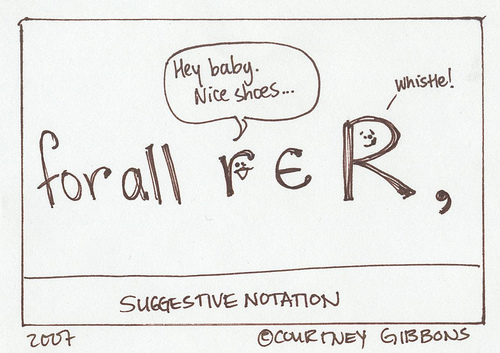
\includegraphics[width=3in]{notation}
\end{center}

\subsection{Common math notation}

\bi
\item $a,~b,~c,~d$:  Real numbers
\bi
\item Examples: 4, $\sqrt{2}$, $\frac{2}{3}$, 3.14159265
\item The set of real numbers is denoted ${\bf R}$ or $\ro$ and
  includes any number ranging from $-\infty$ to $+\infty$.
\item You will often see the expression $a \in \ro$, which means that
  $a$ is a real number.  More correctly, it means that $a$ is in the set of real numbers.
\ei
\item$i,~j,~k,~l$: Integers (whole numbers)
\bi
\item Examples: $\dots, -3, -2, -1, 0, 1, 2, 3, \ldots $
\item The set of integers is denoted $\mathcal{I}$.  Positive integers
  are denoted $\mathcal{I}^+$.  Negative integers are $\mathcal{I}^-$. 
\ei
\item $x,~y,~z$: Variables that can take on varying values.
\item $f,~g,~h$:  Functions of some variable (e.g., $f(x)$)
\item $n$: Commonly denotes some non-specified positive integer.  For
  example, it usually represents the sample size.
\item These are often used in combination:
\bi
\item Indexing: $a_1+a_2 + \ldots + a_i$
\item Functions: $f(x) = a + bx$
\ei
\item Special combinations:
\bi
\item Summation: $\sum_{i=1}^n x_i = x_1+x_2+\ldots+x_n$ \\
\be
  \item $\sum\limits_{i=1}^n c x_i = c \sum\limits_{i=1}^n x_i $
  \item $\sum\limits_{i=1}^n (x_i + y_i) =  \sum\limits_{i=1}^n x_i +
         \sum\limits_{i=1}^n y_i $
  \item $\sum\limits_{i=1}^n c = n c $
  \item $\sum\limits_{i=0}^n i = \sum\limits_{i=1}^n i = \frac{n(n+1)}{2}$
  \item $\sum\limits_{i=1}^n i^2 = \frac{n(n+1)(2n+1)}{6}$
  \item $\sum\limits_{i=1}^n i^3 = (\frac{n(n+1)}{2})^2 = (\sum\limits_{i=0}^n i)^2$
  
  \ee
\item Product: $\prod_{i=1}^n  x_i = x_1\times x_2\times \ldots
  \times x_n$

 \be
  \item $\prod\limits_{i=1}^n c x_i = c^n \prod\limits_{i=1}^n x_i $
  \item $\prod\limits_{i=1}^n (x_i + y_i) =$ a mess 
  \item $\prod\limits_{i=1}^n c = c^n $
  \ee
\ei
\ei


\subsection{Exponents}
\bi
\item $a^3 = a \times a \times a$: ``a to the power of 3'' or ``a to
  the 3rd''.
\item $a^n = a \times a \times \ldots \times a = \prod_{i=1}^na$  
\ei
\noi {\bf Some basic rules that apply at all times}:
\be
\item $a^1 = a$
\item $a^0 = 1$\footnote{Really?  Doesn't this seem a bit strange?
    Ask about it.}
\item $(a^k)^l =a^{kl}$
\item $(ab)^k=a^k \times b^k$
\item $(\frac{a}{b})^k = \frac{a^k}{b^k}$
\item $a^{-1} = \frac{1}{a}$
\item $a^{\frac{1}{2}}=\sqrt{a}$
\item $\sqrt[k]{a} = a^{\frac{1}{k}}$
\ee

\noi {\bf Rules that are true only when $a=b$ (each part has the same ``base'')}:
\bi
\item $a^k \times b^l= a^{k+l}=b^{k+l}$
\item $\frac{a^k}{b^l}=a^{k-l}= b^{k-l}$
\ei


\subsection{Logarithms}

\bi
\item Logarithms are the power required to raise a base to a given
  number: \footnote{Do you really need to know this?  When will you
    ever use this information?} \\
$$y = log_a(x) \qlq a^y = x$$
\item It is helpful to think of the log as the inverse of exponential
  functions.  
$$log_a(a^x) = x$$ 
$$a^{log_a(x)}=x$$
\item In almost all cases you will see logarithms are base 10 or base
  $e$, where $e$ is $euler's constant$.
\be
\item Base 10: $b = log_{10}(a) \iff 10^b = a$ \\
The base 10 logarithm is often simply written as ``$log(x)$" with no
base denoted.
\item Base $e$: $y=log_e(x) \iff e^y = x$ \\
The base $e$ logarithm is referred to as the ``natural'' logarithm and
is usually written as  $ln(x)$.
\item In statistics, you will almost always be working with $ln(x)$.
\ee
\item Some properties of logs:
\be
\item $log_c(ab) = log(a) + log(b)$ Why?:\\
$$ x = log_c(ab) \iff c^x=ab $$
$$\qlq c^{x_1+x_2} = ab, \mbox{  where } x = x_1 + x_2$$
$$\qlq c^{x_1}c^{x_2}=ab \qlq c^{x_1}=a; c^{x_2}=b$$
$$\qlq x_1 = log_c(a); x_2 = log_c(b) $$
$$\qlq log_c(ab) = log_c(a) + log_c(b)$$
\item $log(1/x) = - log(x)$
\item $log(x/y) = log(x) - log(y)$
\item $log(x^y) = ylog(x)$
\item $log(1) = 0$
\item $\ln(e)=1$
\ee
\item You can switch bases as necessary using the following equation:
  $log_b(x) = \frac{log_a(x)}{log_a(b)}$
\item If you see a product of an exponent, you might want to use a log
  to change it into sums:
$$ln(\prod_{i=1}^nae^{x_i}) = ln(ae^{x_1} \cdot ae^{x_2} \cdot ... \cdot ae^{x_n}) = ln(a^n \cdot e^{\sum x_i})$$
$$ ln(a^n) + ln(e^{\sum x_i}) = nln(a) + \sum x_i ln(e) = nln(a) + \sum x_i $$
 
\ei

% Assign the proofs for the above properties as homework.

\subsection{Euler's constant}

\bi
\item Euler's constant is denoted $e$ and is equal to
  $2.71828\ldots$.
\item Like $\pi$, it appears in a surprising number of places in math,
  probability, and statistics.
\bi
\item It is the only number such that the derivative of $e^x$ is equal
  to itself.
\item $e = \llim_{x\to \infty} (1+\frac{1}{x})^x$
\item $e = \sum_{x=0}^\infty\frac{1}{x!}$
\ei
\ei

\subsection{Order of operations}
\bi
\item \textbf{P}lease \textbf{E}xcuse \textbf{M}y \textbf{D}ear \textbf{A}unt \textbf{S}ally 
\item \textbf{P}arentheses \textbf{E}xponents \textbf{M}ultiplication
  \textbf{D}ivision \textbf{A}ddition \textbf{S}ubtraction
\item Example:  $$((1+3)^3)^2 \times 2 + 5 = (4^3)^2 \times 2 + 5$$
$$ =  (64)^2 \times 2 + 5 = 4096  \times 2 + 5 = 8197$$
\ei


\subsection{Coordinate Geometry}
\bi
\item Pairs of numbers represent points: $(x_1, y_1), (x_2, y_2),
  (x_3, y_3), \ldots, (x_n, y_n)$
\item The plot has two axes:
\bi
\item $x$-axis is the horizontal axis at the pottom of the plot
\item $y$-axis is the verticle line on the left hand of the plot
\ei 
\item To plot some point $(x_i, y_i)$:
\bi
\item Move along the x-axis to the point $x_i$ from zero
\item Move up or down to the position of $y_i$ 
\ei
\ei
\begin{center}
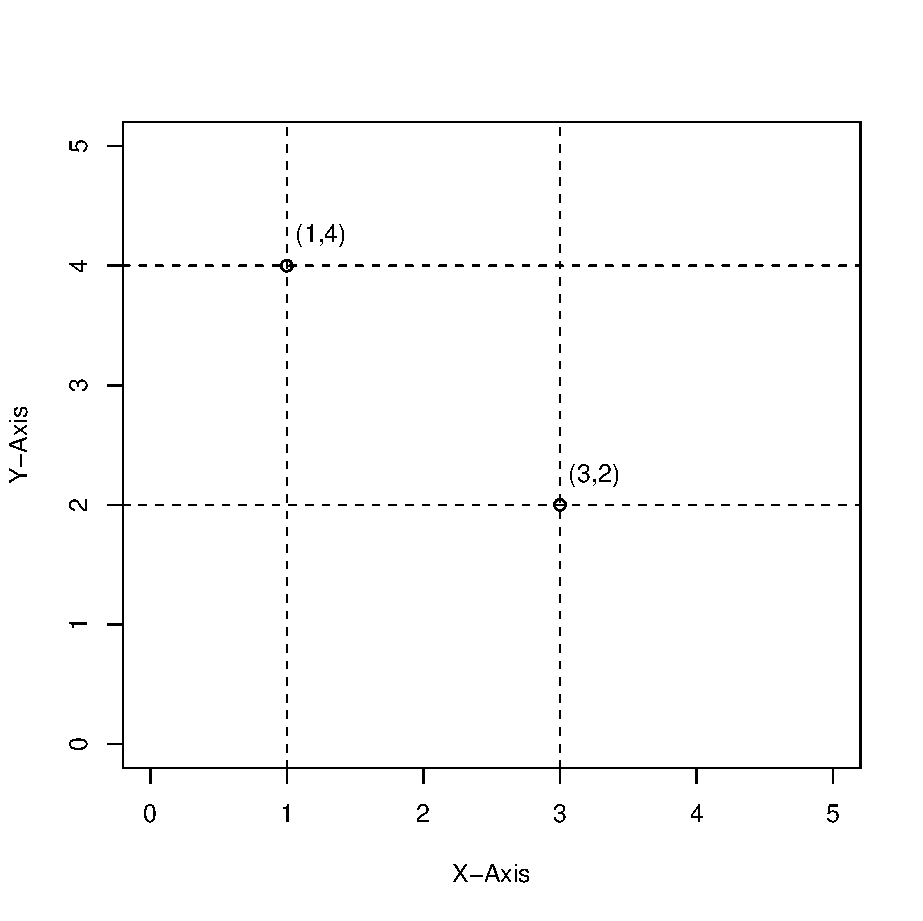
\includegraphics[scale = .8]{graph_example}
\end{center}
% plot(NULL, xlim=c(0,5), ylim=c(0,5), xlab = "X-Axis", ylab = "Y-Axis")
% points(3,2)
% points(1,4)
% abline(v=c(1,3), lty=2)
% abline(h=c(2,4), lty=2)
% text(3+.25,2+.25, "(3,2)")
% text(1+.25,4+.25, "(1,4)")

\subsection{Lines}

\bi
\item The equation for a line will most often be written as:
\be
\item $y=mx + b$ 
\item $y=a+bx$
\item $y=\beta_0 + \beta_1x$
\ee
\item Hardly a day will go by for the next five years when you do not
  encounter (implicitly or explicitly) an equation that looks like
  this.
\item From any two points we can calculate the ``slope'' (e.g., $m$) and
  the ``intercept.''
\bi
\item The slope is the ratio of the differences in the two y pairs and
  the two x pairs (i.e., rise over run)
\item The intercept is the value of the function where $x=0$.  In
  other words, it is the point where the line hits the y-axis.
\ei
\item\textbf{ Example:} ${[2,1], [3,5]}$
\bi
\item$ m = \frac{5-1}{3-2}=4$
\item $1 = 4(2) + b \iff b=1-8=-7$
\ei 
\ei


\section{Functions}
\begin{centering}
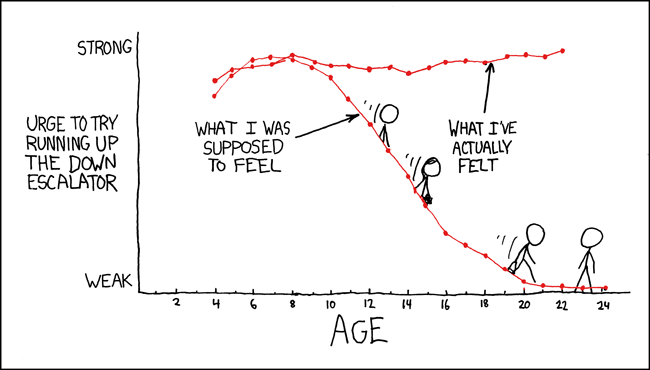
\includegraphics[width=6in]{escalators}
\end{centering}


\subsection{$\ro$ and ${\bf R}^n$}
\bi
\item $\ro$ is the set of all {\bf real} numbers extending from
$-\infty$ to $+\infty$ --- i.e., the real number line.
\item ${\bf R}^n$ is an $n$-dimensional space (often referred to as Euclidean
space), where each of the $n$ axes extends from $-\infty$ to $+\infty$.
\item Examples:
  \be
  \item $\ro$ is a line.
  \item ${\bf R}^2$ is a plane.
  \item ${\bf R}^3$ is a 3-D space.
  \item ${\bf R}^4$ could be 3-D plus time.
  \ee
\item Points in ${\bf R}^n$ are ordered $n$-tuples, where each element
of the $n$-tuple represents the coordinate along that dimension.
\ei


\subsection{Interval Notation for $\ro$}
\bi
\item \pbt{\bf Open interval:} $(a,b)\equiv \{ x\in\ro: a<x<b\}$
\item \pbt{\bf Closed interval:} $[a,b]\equiv \{ x\in\ro: a\le x \le b\}$
\item \pbt{Half open, half closed:} $(a,b]\equiv \{ x\in\ro: a<x\le b\}$
\ei

\subsection{Introduction to Functions}
\bi
\item A {\bf function} (in $\ro$) is a rule or relationship or mapping
or transformation that assigns one and only one number in $\ro$ to each
number in $\ro$.
\item Mapping notation examples
  \be
  \item \pbt{Function of one variable:} $f:\ro\to\ro$
  \item \pbt{Function of two variables:} $f: {\bf R}^2\to\ro$
  \ee
\item Examples:
  \be
  \item $f(x)=x+1$\\
        For each $x$ in $\ro$, $f(x)$ assigns the number $x+1$.
  \item $f(x,y)=x^2+y^2$\\
        For each ordered pair $(x,y)$ in ${\bf R}^2$, $f(x,y)$ assigns
the number $x^2+y^2$.
  \ee
\item Often use one variable $x$ as input and another $y$ as output.\\
Example: $y=x+1$
\item Input variable also called {\bf independent} variable.
Output variable also called {\bf dependent} variable.
\ei

\subsection{Domain and Range}
\bi
\item Some functions are defined only on proper subsets of
  $\rn$.\footnote{What is the point of this?}
\item {\bf Domain}: the set of numbers in $X$ at which $f(x)$ is defined.
\item {\bf Range}: elements of $Y$ assigned by $f(x)$ to elements of
$X$, or $$f(X)=\{ y : y=f(x), x\in X\}$$
Most often used when talking about a function $f:\ro\to\ro$.
 \item Examples:
   \be   
    \item $f(x)=\frac{3}{1+x^2}\quad$ \\[6pt]
  Domain $X=\ro$\\
   Range $f(X)=(0,3]$
%   \parbox{1in}{\,  {\includegraphics[width=1in, angle = 270]{3ovr1x2.eps}}}\\[12pt]

  \item $f(x)=\left\{
    \begin{array}{lcl}
    x+1, &\quad & 1\le x\le 2\\
    0,   &      & x=0\\
    1-x  &      & -2\le x\le -1
    \end{array}
    \right.$\\[6pt]
  Domain $X=[-2,-1]\cup\{0\}\cup[1,2]$\\
  Range $f(X)=[2,3]\cup\{0\}$\\

   \item $f(x)=1/x$\\[6pt]
   Domain $X=\ro-\{0\}$\\
   Range $f(X)=\ro-\{0\}$
 % % \parbox{1.5in}{\, {\includegraphics[width=1in, angle = 270]{1ovrx.eps}}}\\

   \item $f(x,y)=x^2+y^2$\\[6pt]
   Domain $X={\bf R}^2$\\
   Range (or Image) $f(X,Y)={\bf R}^1_+$
 % % \epsfxsize=2.5in
 % % \parbox{2.5in}{\,  {\includegraphics[width=2in, angle = 270]{x2y2.eps}}}
  \ee
\ei

\subsection{Some General Types of Functions}
\bi
\item {\bf Monomials}:  $f(x)=a x^k$\\
$a$ is the coefficient.  $k$ is the degree.\\
Examples: $y=x^2$, $y=-\frac{1}{2}x^3$
\item {\bf Polynomials}: sum of monomials.\\
Examples: $y=-\frac{1}{2}x^3+x^2$, $y=3x+5$\\
The degree of a polynomial is the highest degree of its
monomial terms.  Also, it's often a good idea to write polynomials
with terms in decreasing degree.

\item {\bf Linear}: polynomial of degree 1.\\
 Example: $y=m x + b$, where $m$ is the slope and $b$ is the
 $y$-intercept.
%}\epsfxsize=1in \parbox{1in}{\,
% {\includegraphics[width=.9in, angle = 270]{linear.eps}}}
 \item {\bf Nonlinear}: anything that isn't constant or polynomial of
 degree 1.\\
 Examples:  $y=x^2+2x+1$, $y=\sin(x)$, $y=\ln(x)$, $y=e^x$
%}
%
% \parbox{1in}{\,  {Jacob}}
\item {\bf Quadratic}: a second degree polynomial function.\\
Example: $f(x) = ax^2 + bx + c$
\item Always, always, always, graph your function.
% \item {\bf Rational Functions}: ratio of two polynomials.\\
% Examples: $y=\frac{x}{2}$, $y=\frac{x^2+1}{x^2-2x+1}$
 %\item {\bf Exponential Functions}: Example: $y=2^x$
 %\item {\bf Trigonometric Functions}: Examples: $y=\cos(x)$,
 %$y=3\sin(4x)$

\ei


\subsection{Inverse Functions}
\bi
\item Sometimes we're given a function $y=f(x)$ and we want to find how
$x$ varies as a function of $y$.  That is, we are trying to ``solve
for'' x.  
\item If $f$ is a one-to-one mapping, then it has an inverse.  This
  will usually be denoted as $f^{-1}(x)$.  That means that
  $f^{-1}(f(x)) = x$.
\item A good way to do this is to use algebra to isolate $x$ (your
  independent variable in $f(x)$) on one side of the equation.
\item Examples:  (we want to solve for $x$)
  \be
  \item $y=3x+2 \qlq y-2=3x \qlq x=\frac{1}{3}(y-2)$
  \item $y=3x-4z+2 \quad \lra\quad y+4z-2=3x \qlq
x=\frac{1}{3}(y+4z-2)$
  \item $y=e^x+4 \qlq y-4=e^x \qlq \ln(y-4)=\ln(e^x)
\qlq x=\ln(y-4)$
  \ee
\item Note: the inverse may not not exist.  This is especially likely
  in non-linear functions.
\item Example: We're given the function $y=x^2$ (a parabola).  Solving for
$x$, we get $x=\sqrt{y}$ and $x=-\sqrt{y}$ --- for each value of
$y$, there are two values of $x$. \ei


\subsection{Roots}

\bi 
\item You are going to be spending a lot of time finding
  \textbf{roots} of functions: those values where $f(x) = 0$.
\bi
\item Decision theory/game theory 
\item Dynamic systems
\item Maximum likelihood
\ei
\item Procedure: Given $y=f(x)$, set $y=0$.  Solve for $x$.
\item \textbf{x-intercepts}: Where does the line $f(x) = a + bx$ cross the x-axis?\\
$a+bx = 0 \qlq a = -bx \qlq x = -\frac{a}{b}$
\item \textbf{The ``quadratic equation''}: What is the root of  $f(x) = ax^2 + bx +c$ \\
$x=\frac{-b\pm\sqrt{b^2-4ac}}{2a}$.
\item  \textbf{Factoring}  $f(x)=x^2+3x-4=0 \qlq (x - 1)(x+4) = 0 \qlq
  x=\{1,-4\}$.
\bi
\item\textbf{ FOIL} (\textbf{F}irst \textbf{O}utside\textbf{ I}nside\textbf{ L}ast)
\item The middle term (e.g., $3x$) is the sum of the constants.  The
  final term is the product.
\item If you have $ax^2 - c$, then the factors are of the form
  $(\sqrt{a}x+\sqrt{c})(\sqrt{a}x-\sqrt{c})$
\item If you cannot figure out how to factor, you may need to
  ``complete the square.''  (Google it!)
\ei
\ei




\section{Neighborhoods: Intervals, Disks, and Balls}
\bi
\item In many areas of math, we need a formal construct for what it
means to be ``near" a point $\bf c$ in $\rn$.  This is generally called
the {\bf neighborhood} of $\bf c$ and is represented by an open
interval, disk, or ball, depending on whether $\rn$ is of one, two, or
more dimensions, respectively.
Given the point $c$, these are defined as
  \be
  \item \pbt{{\bf $\eps$-interval} in $\ro$:} $\{ x : |x-c|<\eps \}$ \\
  The open interval $(c-\eps,c+\eps)$.
  \item \pbt{{\bf $\eps$-disk} in ${\bf R}^2$:} $\{\bf x : || x-c ||<\eps\}$\\
  The open interior of the circle centered at $\bf c$ with radius $\eps$.
  \item \pbt{{\bf $\eps$-ball} in $\rn$:} $\{\bf x : || x-c ||<\eps\}$\\
  The open interior of the sphere centered at $\bf c$ with radius $\eps$.
  \ee

\ei


\section {Sets, Sets, and More Sets}

\bi
\item {\bf Interior Point}: The point $\bf x$ is an interior point of
the set $S$ if $\bf x$ is in $S$ and if there is some $\eps$-ball around $\bf x$
that contains only points in $S$.   The {\bf interior} of $S$ is the
collection of all interior points in $S$.  The interior can also be
defined as the union of all open sets in $S$.\\
Example: The interior of the set $\{ (x,y) : x^2+y^2\le 4 \}$ is
$\{ (x,y) : x^2+y^2< 4 \}$ .
\item {\bf Boundary Point}: The point $\bf x$ is a boundary point of the
set $S$ if every $\eps$-ball around $\bf x$ contains both points that are in $S$
and points that are outside $S$.  The {\bf boundary} is the collection
of all boundary points.\\
Example: The boundary of $\{ (x,y) : x^2+y^2\le 4 \}$ is
$\{ (x,y) : x^2+y^2 = 4 \}$.
\item {\bf Open}: A set $S$ is open if for each point $\bf x$
in $S$, there exists an open $\eps$-ball around $\bf x$ completely
contained in $S$.\\
Example: $\{ (x,y) : x^2+y^2<4 \}$
\item {\bf Closed}: A set $S$ is closed if it contains all of its
boundary points.\\
Example: $\{ (x,y) : x^2+y^2\le 4 \}$
\item Note: a set may be neither open nor closed.\\
Example: $\{ (x,y) : 2 < x^2+y^2\le 4 \}$
\item {\bf Complement}: The complement of set $S$ is everything outside
of $S$.\\
Example: The complement of $\{ (x,y) : x^2+y^2\le 4 \}$ is
$\{ (x,y) : x^2+y^2 > 4 \}$.
\item {\bf Closure}: The closure of set $S$ is the smallest closed set
that contains $S$.\\
Example: The closure of $\{ (x,y) : x^2+y^2<4 \}$ is
$\{ (x,y) : x^2+y^2\le 4 \}$
\item {\bf Bounded}: A set $S$ is bounded if it can be contained within
an $\eps$-ball.\\
Examples:  Bounded: any interval that doesn't have $\infty$ or $-\infty$
as endpoints; any disk in a plane with finite radius.  Unbounded: the
set of integers in $\ro$; any ray.
\item {\bf Compact}: A set is compact if and only if it is both closed
and bounded.

\ei




\end{document}




\section{Summation and Product Notation}
\bi
\item \pbt{\bf Summation:}  $\sum\limits_{i=1}^n x_i = x_1+x_2+x_3+\cdots+x_n$
  \be
  \item $\sum\limits_{i=1}^n c x_i = c \sum\limits_{i=1}^n x_i $
  \item $\sum\limits_{i=1}^n (x_i + y_i) =  \sum\limits_{i=1}^n x_i +
         \sum\limits_{i=1}^n y_i $
  \item $\sum\limits_{i=1}^n c = n c $
  \ee

\item \pbt{\bf Product:} $\prod\limits_{i=1}^n x_i = x_1 x_2 x_3 \cdots x_n$

 \be
  \item $\prod\limits_{i=1}^n c x_i = c^n \prod\limits_{i=1}^n x_i $
  \item $\prod\limits_{i=1}^n (x_i + y_i) =$ a mess
  \item $\prod\limits_{i=1}^n c = c^n $
  \ee

\item {\bf Use logs to go between sum, product notation:}

$\log(\prod\limits_{i=1}^n c x_i) =  \sum\limits_{i=1}^n \log (c x_i) = n \log(c) +  \sum\limits_{i=1}^n \log (x_i)$

\ei


\section{Log, Ln, and e}
\bi
\item Relationship of logarithmic and exponential functions: $$
y=\log_a(x) \iff a^y=x$$
The log function can be thought of as an inverse for exponential
functions.  $a$ is referred to as the ``base" of the logarithm.
\item The two most common logarithms are base 10 and base $e$.
  \be
  \item Base 10: $\quad y=\log_{10}(x) \iff 10^y=x$\\
  The base 10 logarithm is often simply written as ``$\log(x)$" with no
base denoted.
  \item Base $e$: $\quad y=\log_e(x) \iff e^y=x$\\
  The base $e$ logarithm is referred to as the ``natural" logarithm and is
  written as ``$\ln(x)$". \epsfxsize=1in
   {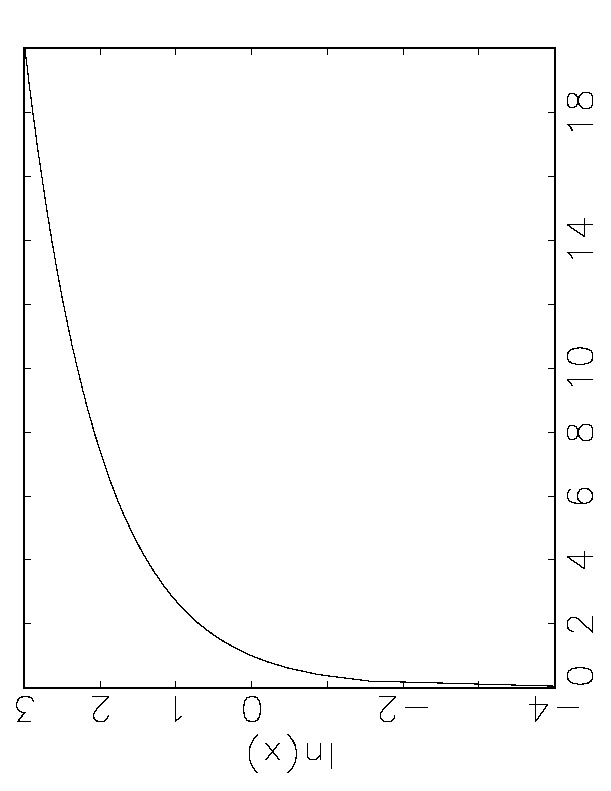
\includegraphics[width=1in, angle = 270]{lnJ}} \,  {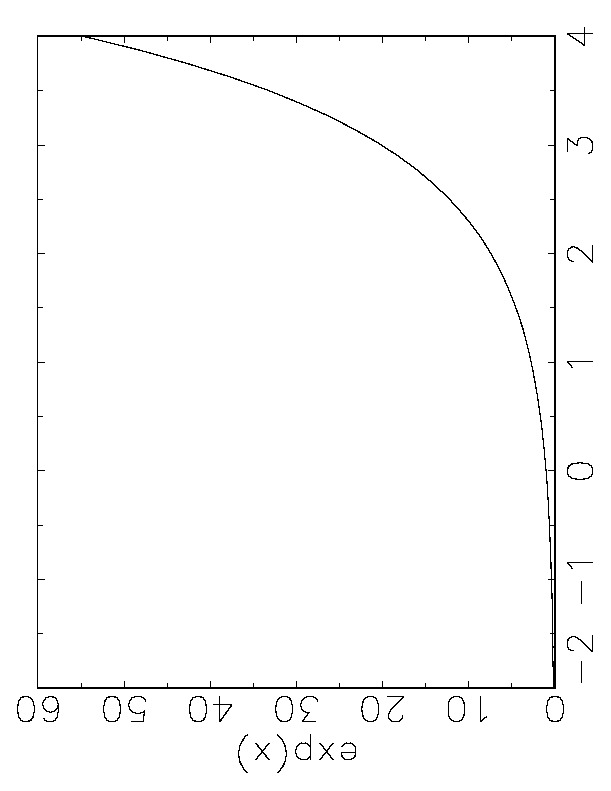
\includegraphics[width=1in, angle = 270]{expJ}}
  \ee

\item $\log_a(a^x)=x$ and $a^{\log_a(x)}=x$
\item Examples:
  \be
  \item $\log(\sqrt{10})=1/2$
  \item $\log(1)=0$
  \item $\log(10)=1$
  \item $\log(100)=2$
  \item $\ln(1)=0$
  \item $\ln(e)=1$
  \ee
\item Properties of exponential functions:
  \be
  \item $a^x a^y = a^{x+y}$
  \item $a^{-x} = 1/a^x$
  \item $a^x/a^y = a^{x-y}$
  \item $(a^x)^y = a^{x y}$
  \item $a^0 = 1$
  \ee
\item Properties of logarithmic functions (any base):
  \be
  \item $\log(x y)=\log(x)+\log(y)$
  \item $\log(1/x)=-\log(x)$
  \item $\log(x/y)=\log(x)-\log(y)$
  \item $\log(x^y)=y\log(x)$
  \item $\log(1)=0$
  \ee
\item Use the change of base formula to switch bases as necessary: $\log_b(x) = \log_a(x)/\log_a(b)$ 
\ei
